In this chapter we present the JS-QL framework. The framework offers the possibility for developers to write application-specific queries to check for certain program properties. More specific, it tries to offer a solution to developers who want to test their applications for vulnerabilities by writing and enforcing security policies for them. The framework consists of three main parts: 
\begin{enumerate}
\item \textit{The JS-QL query language}: Short for \textbf{J}ava\textbf{S}cript \textbf{Q}uery \textbf{L}anguage. This is the domain-specific language in which users can express all kinds of security policies. An overview of the language is given in section \ref{sec:JSQLlanguage}.
\item \textit{The matching engine}: This is the core of the framework. It matches the user-defined query against states of the JIPDA abstract state graph, capturing and unifying all the relevant information. This engine can be configured to behave differently for certain queries, as will be discussed in section \ref{subsec:TypesOfQueries}.
\item \textit{The graphical user interface}: The user interface provides the infrastructure for the developer to interact with the framework. It contains a section where users can specify the input program and security policy, a graphical component representing the abstract state graph corresponding to the input program and a visual and textual representation of the query results. The textual representation allows developers to inspect the captured variables, a handy feature when these variables are compound data structures. A brief overview of the user interface will be given in section \ref{sec:GUI}.
\end{enumerate}

\section{The JS-QL query language}
\label{sec:JSQLlanguage}

The abstract state graph obtained from the JIPDA analysis is a perfect starting point to inspect a program for certain characteristics and security vulnerabilities. In chapter \ref{ch:Overview} we motivated our choise to design an internal DSL to query for specific (sequences of) states in this graph, with the aim to discover program patterns that might lead to violations of user-defined security policies. The language constructs are built to make it easy for the user to specify which kind of pattern he wishes to detect. The rest of this section presents all facets of the JS-QL language: Section \ref{subsec:Syntax} discusses all constructs of the language and gives an in-depth explanation on how to use them in a correct way. As different security policies require different traversals of the state graph, more than one type of query is needed. We discuss the difference between several query types in section \ref{subsec:TypesOfQueries}. In order to have an effective query language, we must allow the user to create compound queries out of the available language constructs. Section \ref{subsec:DefiningPolicies} shows how this can be done within the framework.

\subsection{JS-QL syntax}
\label{subsec:Syntax}
 In this section we will discuss the available constructs and syntax of the JS-QL language. The examples in this section will be simplistic and will demonstrate how each construct works. They will therefore not always represent an actual security policy, but will rather serve as a guideline for using these constructs.

%Entry point
\subsubsection{The entry point}
As our language is an internal DSL, meaning that it is embedded in a host language, the host language has to provide an entry point from where we can start using the JS-QL language. We chose to map this point to the \texttt{G} object, which is short for \textbf{G}raph. This implies that all query patterns in JS-QL will start from this object. A simple example is seen in \ref{lst:entryPoint}, where the first state of the graph is matched.

\begin{lstlisting}[label={lst:entryPoint},language=JSQL,caption=Matching the first state starting from entry point \texttt{G},mathescape=true]  % float=t?

//Match the first state of the graph
G.state()
\end{lstlisting}

\subsubsection{State}
the \texttt{state} construct is the single most basic element of the language. It matches any state in the graph, but doesn't provide much information on its own. Nevertheless is it the most important building block of the language, as it can be used to construct higher-level queries and predicates. States can be made more precise and expressive by parametrizing them with \textit{state constraints}, but in order to know what we can query for, we will first give a short overview of what information is available in which states. To get a more detailed explanation on what each piece of information represents, we refer to the section about flow graphs (\ref{subsec:FlowGraphs}). Table \ref{tab:InfoPerState} indicates what information is available in which type of state. The table also shows which keyword is used to represent the information is that is in embodied in the states.

\begin{table}[!h]
\centering
\caption*{
  \centering
  	\begin{tabular}{| l | c |}
  	\hline
  	\multicolumn{2}{ |c| }{Legend} \\
  	\hline
  	Evaluation state & $E$  \\
  	Continuation state & $K$  \\
  	Return state & $R_t$  \\
  	Result state & $R_s$  \\
  	All states & $A$  \\
  	\hline
  	\end{tabular}
  	%$E$ = EvalState, $K$ = KontState, $R_t$ = ReturnState, $R_s$ = ResultState, $A$ = All states
  }
  \begin{tabular}{| l | l | c |}
  \hline
  State property & Available in states & Keyword\\
  \hline
  Node & $E$ & node\\
  Meta continuation & $A$ & kont\\
  Local continuation & $A$ & lkont\\
  Binding environment & $E$ & benv\\
  Store & $A$ & store\\
  Value & $K$ $R_t$ $R_s$ & value\\ \hline \hline
  Identifier & $A$ & \_id\\
  Successors & $A$ & \_successors \\
  \hline

  \end{tabular}
  
  \caption{Information in the states of the abstract state graph}
  \label{tab:InfoPerState}
\end{table}

Note that the framework also supports the usage of the identifier and successors of a state, but it is very uncommon to use them, as they are semantically irrelevant to queries. The identifier of a state would only be relevant when a query is matched in that exact state. When this is the case, the state gets marked in the visual graph representation and all query information is then contained in that state. To retrieve the information, one simply has to click the state to inspect all variable values. Successors also contain few additional information, as all direct successors of a state are already made explicit in the state graph. A use case for the use of the successors keyword could be to find all states after which some branching occurs. This could then be specified as a JS-QL query which captures the successors array in a variable \texttt{?succArr}, and then filters the results to only contain the states with the length of \texttt{?succArr} strictly greater than 1.

To understand how we can parametrize states, we first have to know how to define variables in JS-QL. Variables in JS-QL are strings, starting with a \texttt{?}. The fact that we use strings comes from the embedded nature of our language: If we were to specify variables as literals, the host language would complaint that it doesn't recognize the literal. Listing \ref{lst:stringVariables} illustrates this.

\begin{lstlisting}[label={lst:stringVariables},language=JSQL,caption=Defining variables in JS-QL,mathescape=true]  % float=t?

//Capture the 'type' property of the node in variable '?nType'
G.state({ node : { type: '?nType' }})
//Exception: ?nType is not recognized by the host language
G.state({ node : { type: ?nType }}) 
\end{lstlisting}

As the example might already indicate, JS-QL deconstructs state properties as nested key-value pairs. In this way, each part of information can be captured in a variable. The key indicates the property the user wishes to match whereas the value can be one of three things:
\begin{enumerate}
\item A \textit{variable}. When placing a variable as the value in a key-value pair in JS-QL, that variable gets bound to the key's corresponding value in the JIPDA state. The '?nType' variable in the example above gets bound to the value of \texttt{type}, which in this case corresponds with the type of the AST \texttt{node} for the currently matched state.
\item A \textit{nested map} which further deconstructs the current property. The example above does this by further deconstructing the \texttt{node} property of a state (which represents the corresponding AST node) in order to reach the \texttt{type} of that node and store it in a variable. It is obvious that this is most used to match specific AST nodes.
\item A \textit{literal}. Literals are mostly used to filter the states to be matched. When applying this to the example above, the '?nType' variable could be replaced by the literal 'ExpressionStatement' for example. Note that the question mark (\texttt{?}) is omitted. The resulting query would then only match a state having the \texttt{type} of its corresponding AST \texttt{node} equal to 'ExpressionStatement'.
\end{enumerate}

%Kort door de bocht?
\noindent States can thus be parametrized by matching the keywords displayed in table \ref{tab:InfoPerState} as keys with values that can be variables, literals or nested maps. It is obvious that queries matching single-state patterns aren't quite qualified as being security policies. JS-QL therefore allows users to specify sequences of states as a query. When checking the state graph against this query, all states in the query pattern need to be matched one after another. When a state in the query pattern is encountered that doesn't match the current state in the state graph, the matching process is aborted for the current path that is investigated in the state graph. Consider the following query:

\begin{lstlisting}[label={lst:Unification},language=JSQL,caption=Unification in JS-QL,mathescape=true]  % float=t?

G.state({ node : { type: '?tpe' }})
 .state({ node : { type: '?tpe' }})
\end{lstlisting}

\noindent We immediately see that the variable \texttt{?tpe} occurs twice in the query. This can be done on purpose to achieve \textit{unification}. Unification simply means that two variables with the same name have to contain the same value. After executiong the first line, the first state in the graph is matched (if it has the \texttt{node} property) and the variable \texttt{?tpe} is bound to the type of the node. The matching engine then proceeds to the next state in both the query and the state graph. If the next state again has the \texttt{node} property with the same type as already bound to \texttt{tpe}, the unification process has succeeded and the whole query will match. If the node type of the next state isn't equal to the value already bound to \texttt{?tpe}, or if that state doesn't have a \texttt{node} property, there is no match. The results of a successfully matched query will be the set of all possible \textit{substitutions}, together with the identifier of the state where the last element of the query matched. Figure \ref{fig:Unification} gives a simplistic visual representation of this process for the query listed in listing \ref{lst:Unification}. For the graph on the left-hand side, the query is fully matched by successfully unifying the the type of the first and second state. In contrast, the graph on the right-hand side will not produce a match as $\{$\texttt{?tpe} $:$ 'ExpressionStatement'$\}$ can not be unified with $\{$\texttt{?tpe} $:$ 'AssignExpression'$\}$.

\begin{figure}[!ht]
    \centering
      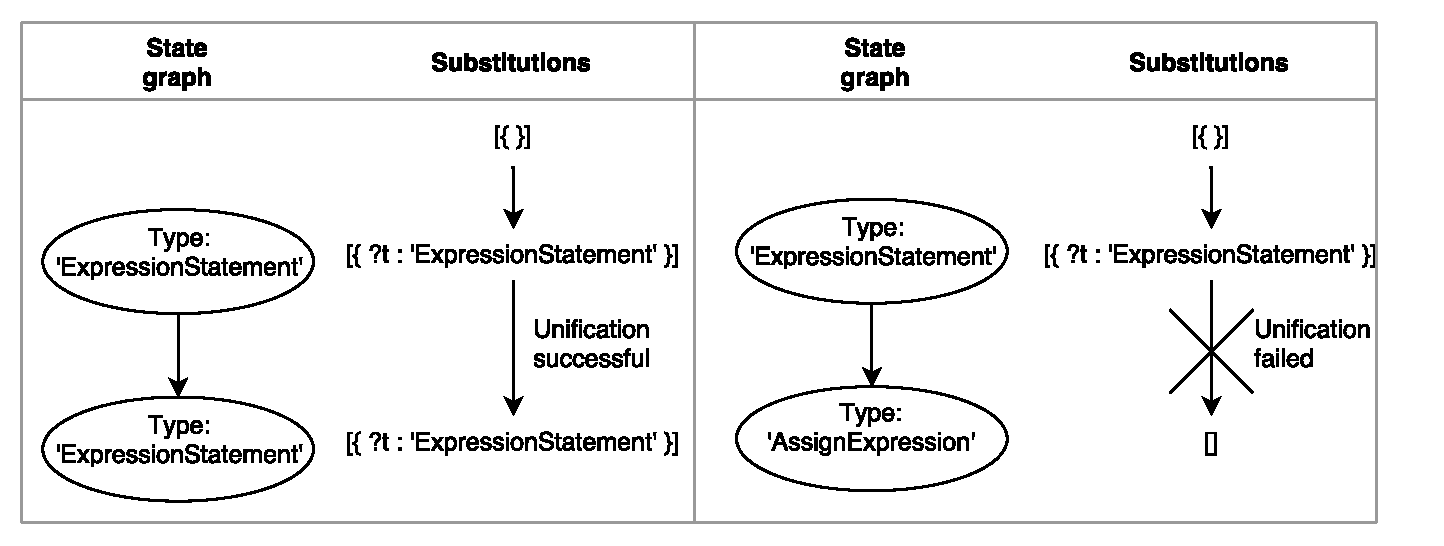
\includegraphics[width=1\textwidth]{images/Unification} 
      \caption{Visual representation of the unification process}
    \label{fig:Unification}
\end{figure}

%Opmerken dat we nu slechts aan het matchen zijn vanaf het begin van de graph, wat als we iets ERGENS in de code willen detecten?
%TODO: translate variables starting with ! to ?__TMP__

%state (+types)
%unification uitleggen tesamen met parametrization + als niet matcht overslaan (tekening van match)


%THIS
%props -> motiveren waarom andere kant
%filters
%lookup
%not
%wildcard
%star
\subsection{Types of queries}
\label{subsec:TypesOfQueries}
%forward
%backward
%Universal
%existential
\subsection{Defining policies}
\label{subsec:DefiningPolicies}
%predikaten en queries
%recursie!
%Policies omgezet naar automaton -> dan naar query engine
\section{The matching engine} 
\label{sec:matchingEngine} %algo uitleggen
% Paper uitleggen met automaton enzovoort enzoverder
\section{The graphical user interface} 
\label{sec:GUI}
